%%%%%%%%%%%%%%%%%%%%%%%%%%%%%%%%%%%%%%%%%%%%%%%%%%%%%%%%%%%%%%%%%%%%%%%%%%%%%%%%
%2345678901234567890123456789012345678901234567890123456789012345678901234567890
%        1         2         3         4         5         6         7         8
\documentclass[letterpaper, 10 pt, conference]{ieeeconf}  % Comment this line out
% if you need a4paper
%\documentclass[a4paper, 10pt, conference]{ieeeconf}      % Use this line for a4

\usepackage{float}
% paper
% uso paquete bookmark para tener bien los outlines.
\usepackage{bookmark}

% Configuro el idioma.
\usepackage[utf8]{inputenc} % Importante para mantener acentos.
\usepackage[spanish, activeacute]{babel} % Requiere: texlive-lang-spanish. Por primera vez hay que ejecutar: texconfig init> log

% Paquete para poder usar acentos en $$.
\usepackage{mathtools}
%\setmathfont{XITS math}

\usepackage{tikz}
\usetikzlibrary{shapes.misc, positioning, shapes.geometric, arrows.meta}

\usepackage{siunitx}

% package to get \url
\usepackage{hyperref}
\hypersetup{
  colorlinks=true,
  linkcolor=magenta,
  filecolor=magenta,
  citecolor=magenta,      
  urlcolor=magenta,
}

% Graficos electrónicos
\usepackage{circuitikz}

\IEEEoverridecommandlockouts                              % This command is only
% needed if you want to
% use the \thanks command
\overrideIEEEmargins
% See the \addtolength command later in the file to balance the column lengths
% on the last page of the document

\usepackage{graphicx}
\usepackage{graphics}

% styling for matlab/octave code.
\usepackage{matlab-prettifier}
% Configuracion, con esto puede agregar ñ.
\lstset{
  literate={ñ}{{\~n}}1
}

% The following packages can be found on http:\\www.ctan.org
%\usepackage{graphics} % for pdf, bitmapped graphics files
%\usepackage{epsfig} % for postscript graphics files
%\usepackage{mathptmx} % assumes new font selection scheme installed
%\usepackage{times} % assumes new font selection scheme installed
\usepackage{amsmath} % assumes amsmath package installed
%\usepackage{amssymb}  % assumes amsmath package installed

\title{\LARGE \bf Laboratorio N° 4}

\author{
  Tom\'as Vidal\\
  {\it Circuitos Electrónicos 1}\\
  {\it Facultad de Ingenier\'ia, UNLP, La Plata, Argentina.}\\
  {\it 20 de Julio, 2024.}
}                                            % <-this % stops a space


% comienzo

% INTRO

% Figura
\newcommand{\image}[2] {
  \begin{figure}[H]
    \centering
    \includegraphics[width=0.43\textwidth]{./#1.png}
    \caption{#2}
    \label{fig:#1}
  \end{figure}
}

% Codigo
% \begin{lstlisting}[style=Matlab-editor]
% % el código va aca
% dispc("HELLO WORLD");
% \end{lstlisting}

\begin{document}
\maketitle
\thispagestyle{empty}
\pagestyle{empty}

\section{Introducción}
Se resuelven de manera analítica las consignas presentadas en el laboratorio 4 de circuitos electrónicos I; posteriormente se muestran los resultados de las mediciones hechas del mismo y las conclusiones.

\section{Topologías}
En el circuito presentado (fig. \ref{pic:circuito_presentado}) se pueden definir dos topologías: \ref{pic:topologia1} y \ref{pic:topologia2}. A continuación se hacen análisis sobre las dos.

\begin{figure}[H]
 \centering
 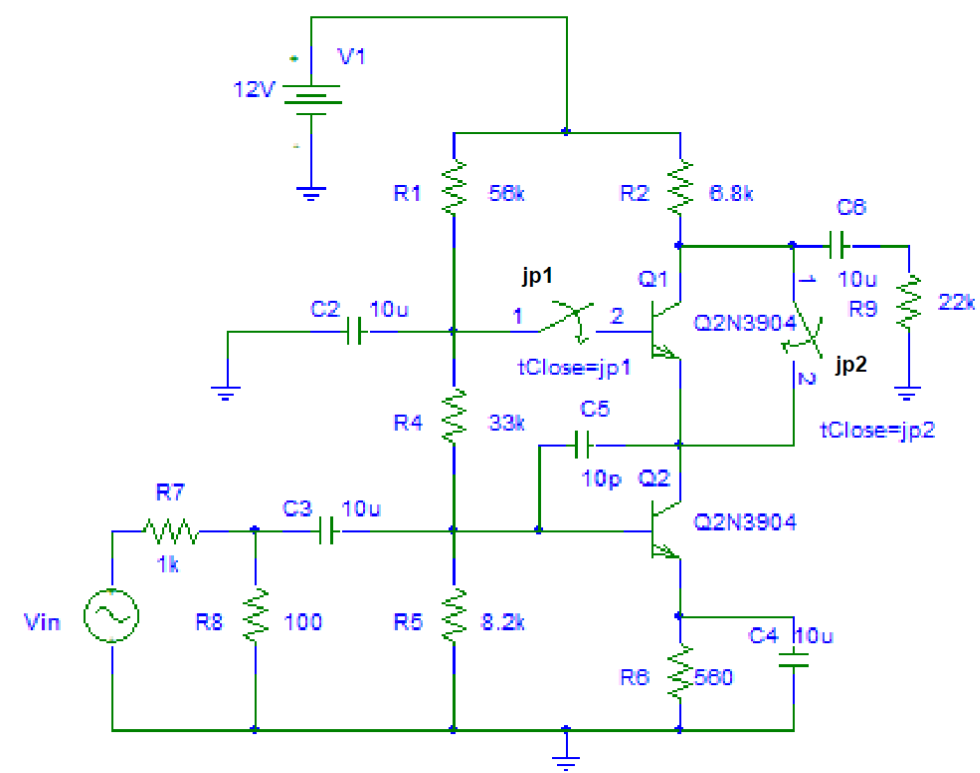
\includegraphics[width=0.43\textwidth]{./Imagenes/circuito_presentado.png}
 \caption{Circuito dado}
 \label{pic:circuito_presentado}
\end{figure}

\begin{figure}[H]
 \centering
 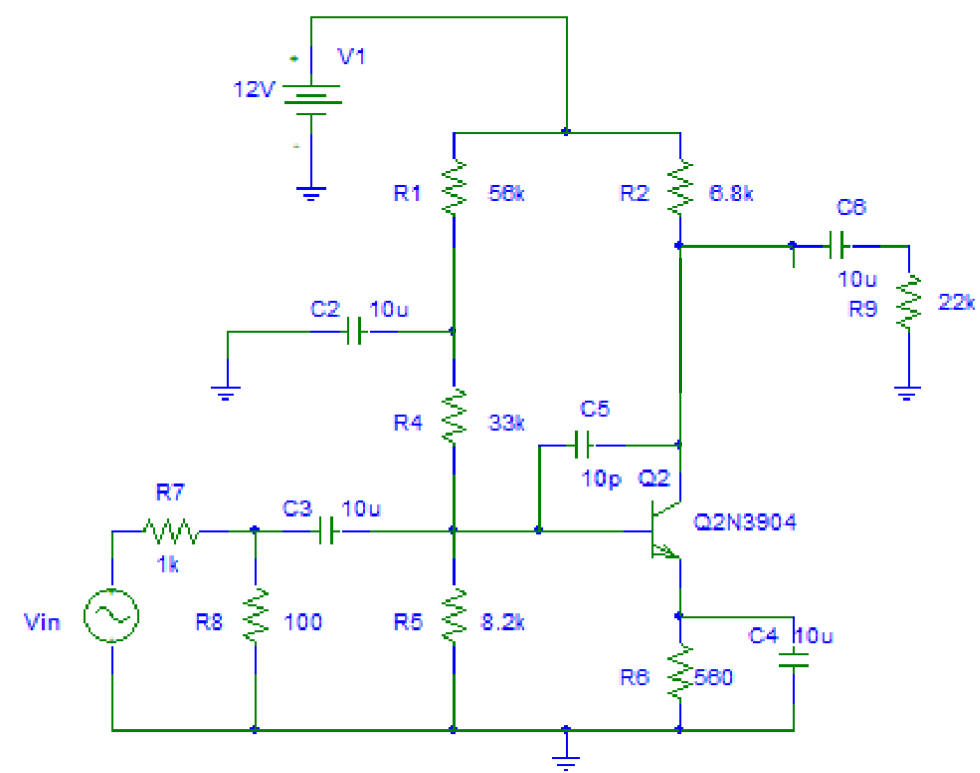
\includegraphics[width=0.43\textwidth]{./Imagenes/topologia1.png}
 \caption{Topología 1}
 \label{pic:topologia1}
\end{figure}

\begin{figure}[H]
 \centering
 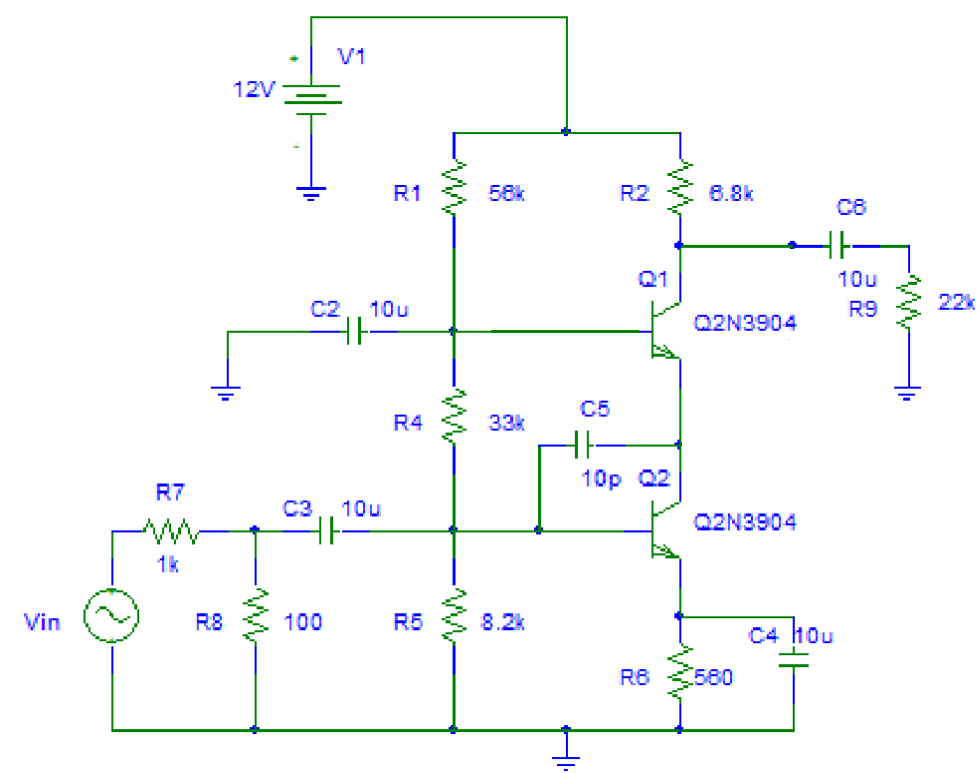
\includegraphics[width=0.43\textwidth]{./Imagenes/topologia2.png}
 \caption{Topología 2}
 \label{pic:topologia2}
\end{figure}

\section{Topología 1}
Esta topología se presenta cuando en el circuito dado, jp1 y jp2 se encuentran abierto y cerrado respectivamente. Es basicamente un BJT con polarización universal en configuración de emisor común.
\subsection{Análisis en DC}
Se encuentra una corriente de polarización $I_{cq} \cong \qty{521}{\micro\ampere}$.

\begin{figure}[H]
 \centering
 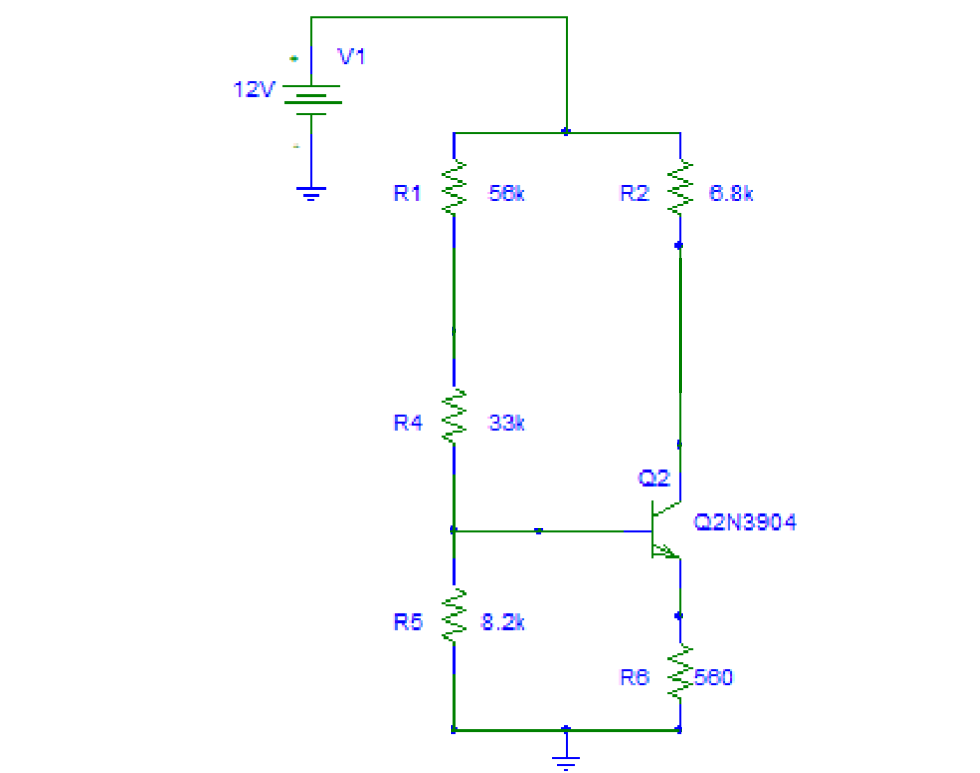
\includegraphics[width=0.43\textwidth]{./Imagenes/topologia1_dc.png}
 \caption{Topología 2 análisis en DC}
\end{figure}

\subsection{Análisis frecuencias medias}
Los parámetros del modelo del BJT en base a la polarización son: $g_m \cong \qty{0.0209}{\siemens}$ y $r_{\pi} \cong \qty{9.5912}{\kilo\ohm}$. Y se obtiene una ganancia de tensión: $A_v \cong -9.6226$

\begin{figure}[H]
 \centering
 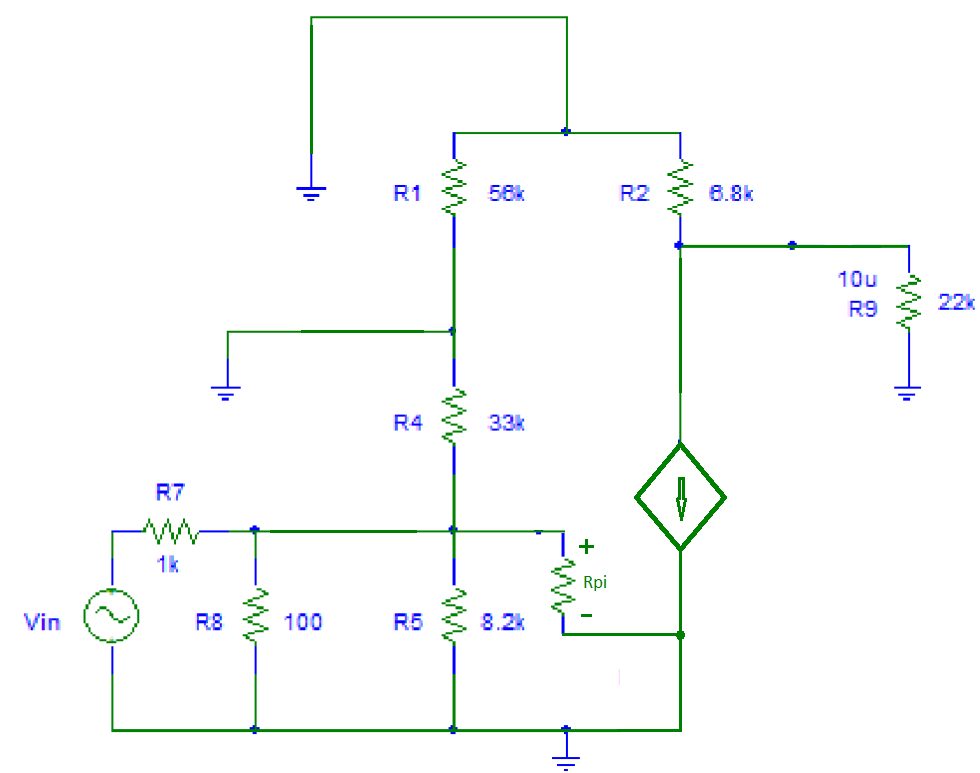
\includegraphics[width=0.43\textwidth]{./Imagenes/topologia1_fm.png}
 \caption{Topología 2 análisis en frecuencias medias}
\end{figure}

\subsection{Análisis frecuencias altas}
El análisis de altas frecuencias es para encontrar el polo dominante, entonces se aproxima el sistema a uno de orden 1, por lo que este polo define la frecuencia de corte. Para hallar esta frecuencia se emplea el método de las constantes de tiempo. Considerando las impedancias ``vistas'' por $C_{\pi}$ y $C_{\mu}$ como $R_{\pi} \cong \qty{88.8374}{\ohm}$ y $R_{\mu} \cong \qty{14.906}{\kilo\ohm}$ respectivamente. Por lo que $\omega_{H1} \cong \frac{1}{ C_{\mu}R_{\mu} + C_{\pi}R_{\pi} } \cong \qty{8.9578}{\mega\radian\per\second}$ y $f_{H1} \cong \qty{1.4257}{\mega\hertz}$

\begin{figure}[H]
 \centering
 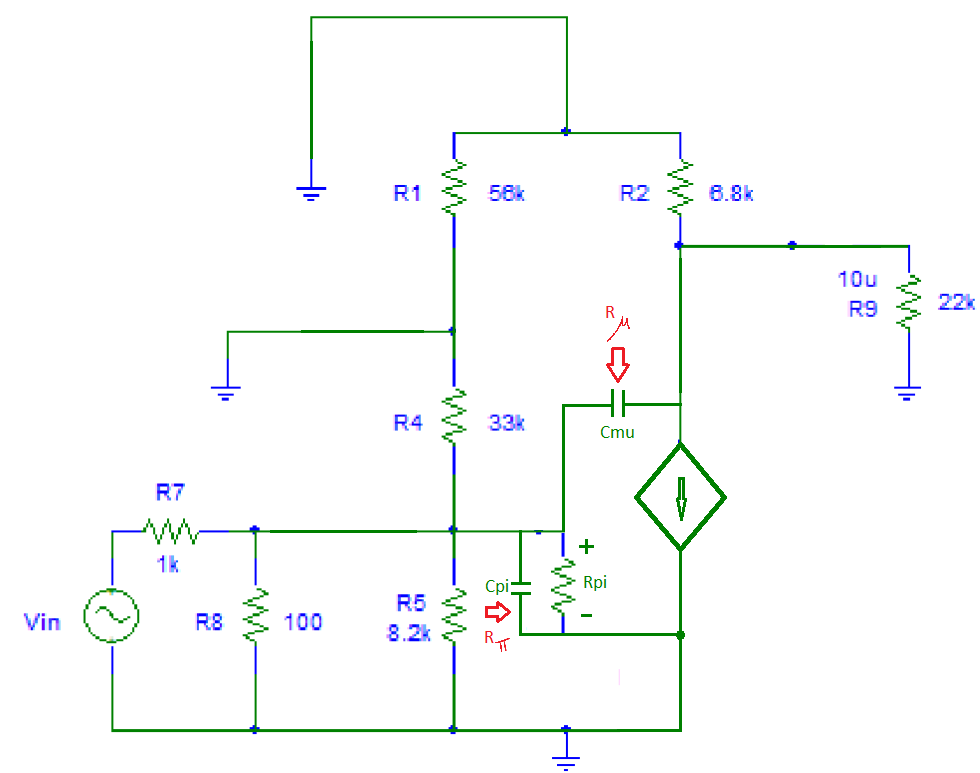
\includegraphics[width=0.43\textwidth]{./Imagenes/topologia1_fa.png}
 \caption{Topología 1 análisis en frecuencias altas}
\end{figure}

\section{Topología 2}
Esta topología se presenta cuando en el circuito dado, jp2 y jp1 se encuentran abierto y cerrado respectivamente. El circuito que queda es un cascode
\subsection{Análisis en DC}
Se encuentra una corriente de polarización $I_{cq} \cong \qty{521}{\micro\ampere}$. La polarización es exactamente la misma para ambos BJT.

\begin{figure}[H]
 \centering
 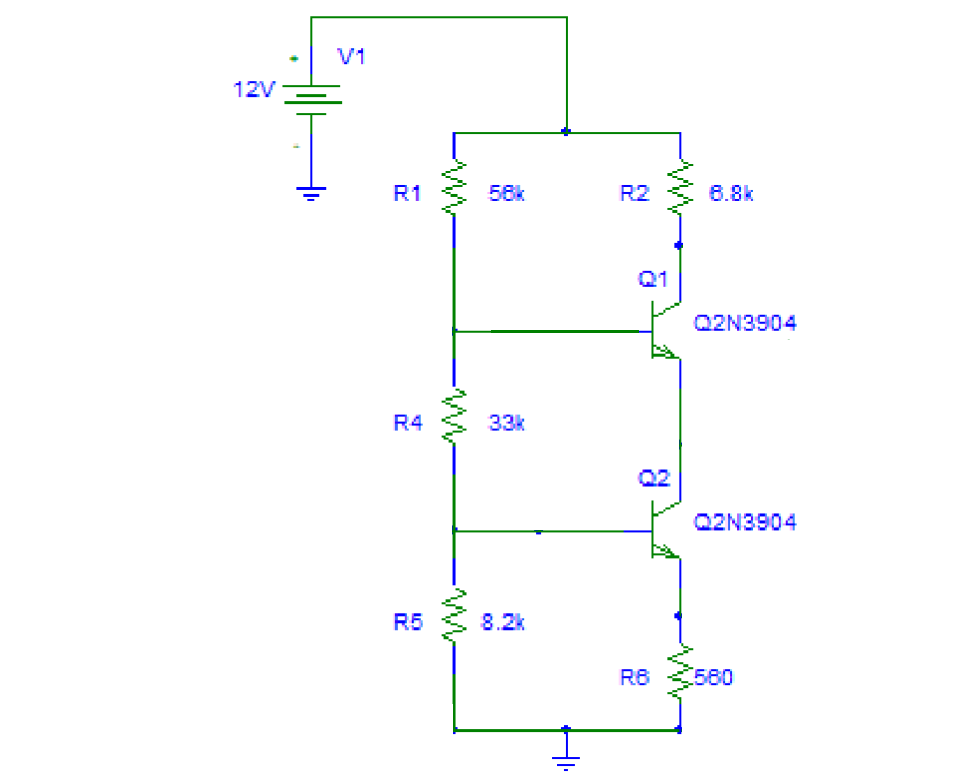
\includegraphics[width=0.43\textwidth]{./Imagenes/topologia2_dc.png}
 \caption{Topología 2 análisis en DC}
\end{figure}

\subsection{Análisis frecuencias medias}
Los parámetros del modelo del BJT en base a la polarización son: $g_m \cong \qty{0.0209}{\siemens}$ y $r_{\pi} \cong \qty{9.5912}{\kilo\ohm}$. Y se obtiene una ganancia de tensión: $A_v \cong -9.6710$.

\begin{figure}[H]
 \centering
 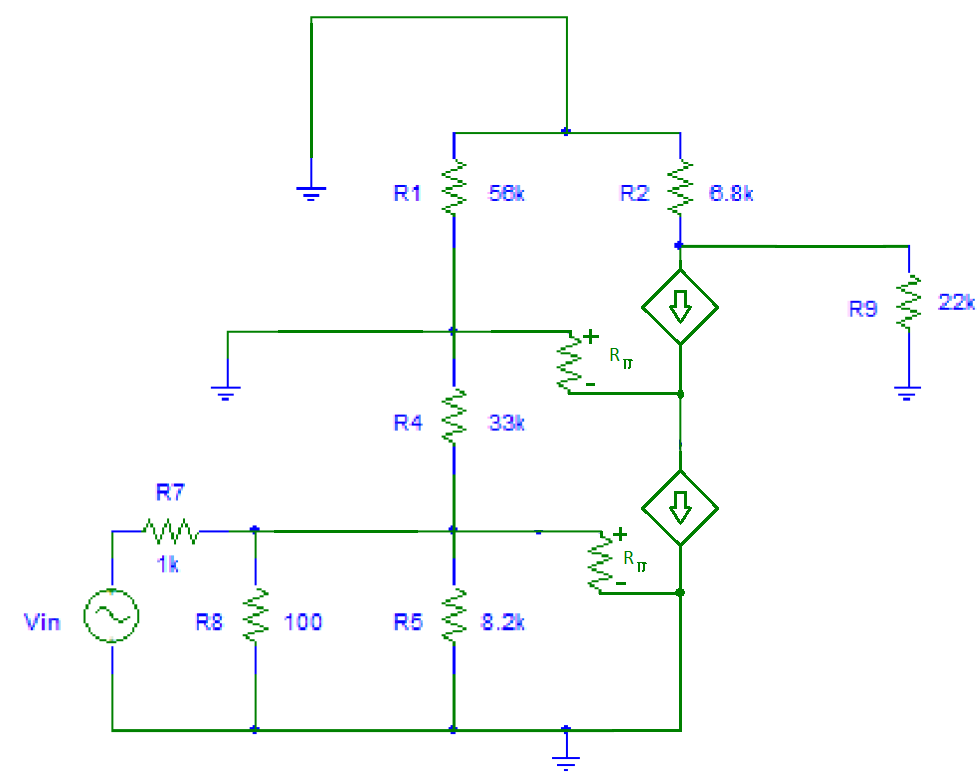
\includegraphics[width=0.43\textwidth]{./Imagenes/topologia2_fm.png}
 \caption{Topología 2 análisis en frecuencias medias}
\end{figure}

\subsection{Análisis frecuencias altas}
Considerando las impedancias ``vistas'' por las capacidades $C_{\pi}$ y $C_{\mu}$ como $R_{\pi1} \cong \qty{88.8374}{\ohm}$, $R_{\pi2} \cong \qty{47.7172}{\ohm}$, $R_{\mu1} \cong \qty{224.9501}{\ohm}$ y $R_{\mu2} \cong \qty{2.3952}{\kilo\ohm}$. Por lo que $\omega_{H2} \cong \frac{1}{ C_{\mu}R_{\mu1} + C_{\mu}R_{\mu2} + C_{\pi}R_{\pi1} + C_{\pi}R_{\pi2} } \cong \qty{11.058}{\mega\radian\per\second}$ y $f_{H2} \cong \qty{1.7600}{\mega\hertz}$

\begin{figure}[H]
 \centering
 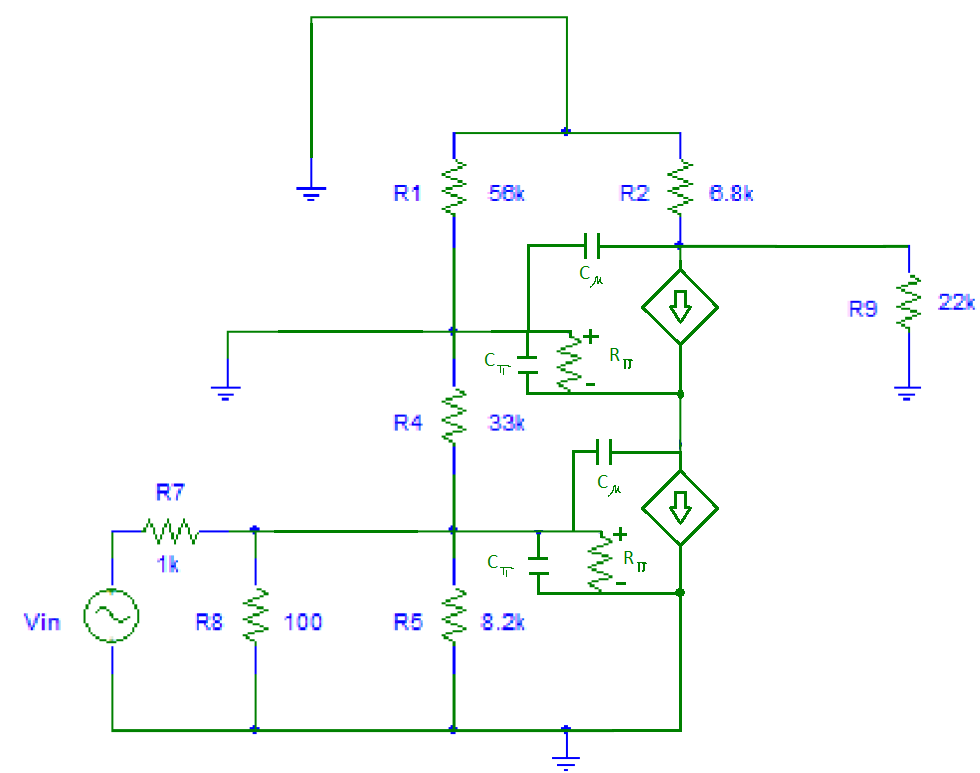
\includegraphics[width=0.43\textwidth]{./Imagenes/topologia2_fa.png}
 \caption{Topología 2 análisis en frecuencias altas}
\end{figure}

\section{Resultados de las mediciones}

 \begin{table}[H]
   \centering
   \begin{tabular}{|lll|ll|}
     \hline
     \multicolumn{3}{|c|}{Analítico}                                                    & \multicolumn{2}{c|}{Medido}                      \\ \hline
     \multicolumn{1}{|l|}{Topologia}  & \multicolumn{1}{l|}{$f_H \left[MHz\right]$}  & $t_r \left[\mu S\right]$ & \multicolumn{1}{l|}{$f_H \left[MHz\right]$} & $t_r \left[\mu  S\right]$ \\ \hline
     \multicolumn{1}{|l|}{1}          & \multicolumn{1}{l|}{1.4257}       & 245         & \multicolumn{1}{l|}{1.5}           & 300         \\ \hline
     \multicolumn{1}{|l|}{2}          & \multicolumn{1}{l|}{1.7600}       & 198         & \multicolumn{1}{l|}{1.55}          & 260         \\ \hline
   \end{tabular}
 \end{table}

\section{Conclusiones}
La topología de cascode tiene mayor ancho de banda, como se puede observar en los cálculos y las mediciones. Aunque las mediciones no son exactamente iguales a lo esperado se acercan lo suficiente, con errores relativos de $f_H$ de 5\% y 11\% para las topologías 1 y 2 respectivamente. La diferencia es más notoria con el tiempo $t_r$, 18\% y 24\% de error relativo; pero probablemente la causa de tanta diferencia sea la forma en cómo se hicieron las mediciones, más que en la discrepancia de lo teórico con lo real.

\end{document}
